\documentclass[aspectratio=169,11pt]{beamer}

% -------------------------
% Tema (puedes cambiarlo)
% -------------------------
\usetheme{Madrid}
\usecolortheme{dolphin}

% -------------------------
% Paquetes
% -------------------------
\usepackage[utf8]{inputenc}
\usepackage[T1]{fontenc}
\usepackage[spanish]{babel}
\usepackage{graphicx}
\usepackage{booktabs}
\usepackage{array}
\usepackage{ragged2e}
\usepackage{hyperref}
\usepackage{caption}

% -------------------------
% Configuración estética
% -------------------------
\setbeamertemplate{navigation symbols}{}
\setlength{\parskip}{4pt}
\justifying

% -------------------------
% Título
% -------------------------
\title{Transmisión de la política monetaria y dinámica inflacionaria en Colombia}
\subtitle{Evidencia empírica mediante un VARX(2)}
\author{Santiago Tupaz}
\date{\today}

% -------------------------
% Helpers
% -------------------------
\newcommand{\figplaceholder}[2]{%
\begin{figure}
  \centering
  \fbox{\parbox[c][0.42\textheight][c]{0.92\textwidth}{\centering \Large #1\\ \vspace{6pt}\normalsize Ruta: \texttt{#2}}}
\end{figure}
}

\begin{document}

% =========================
% Portada
% =========================
\begin{frame}
  \titlepage
\end{frame}

% =========================
% Agenda
% =========================
\begin{frame}{Estructura}
\begin{itemize}
  \item Motivación y pregunta
  \item Datos y transformaciones
  \item Evidencia descriptiva
  \item Metodología: VARX(2) y diagnóstico
  \item Resultados: IRFs y FEVD
  \item Pronóstico y validación fuera de muestra
  \item Conclusiones
\end{itemize}
\end{frame}

% =========================
% Motivación
% =========================
\begin{frame}{Motivación}
\begin{itemize}
  \item La inflación persistente deteriora el poder adquisitivo e incrementa incertidumbre macroeconómica.
  \item Bajo metas de inflación, la tasa de interés es el instrumento central de política.
  \item En economías abiertas, choques externos y el canal cambiario pueden amplificar la dinámica inflacionaria.
\end{itemize}
\end{frame}

% =========================
% Pregunta y objetivo
% =========================
\begin{frame}{Pregunta y objetivo}
\textbf{Pregunta:} ¿En qué medida choques monetarios (DTF) y financieros (TRM), junto con actividad (ISE), afectan la inflación anual en Colombia?

\vspace{8pt}
\textbf{Objetivo:}
\begin{itemize}
  \item Estimar un \textbf{VARX(2)} con bloque endógeno \{inflación, TRM, ISE, DTF\}
  \item Controlar choques externos con exógenas \{inflación EE.UU., Brent\}
  \item Evaluar dinámica (IRF/FEVD) y desempeño predictivo (forecast/expanding window)
\end{itemize}
\end{frame}

% =========================
% Datos
% =========================
\begin{frame}{Datos y fuentes}
\begin{itemize}
  \item Inflación Colombia: variación log interanual del IPC (DANE / BanRep, según tu extracción)
  \item TRM: promedio mensual (Banco de la República)
  \item DTF / CDT 90 días: tasa promedio mensual (Banco de la República)
  \item ISE desestacionalizado: DANE
  \item Exógenas: Inflación EE.UU. (CPIAUCSL, FRED) y Brent (DCOILBRENTEU, FRED)
\end{itemize}
\vspace{6pt}
\textit{Frecuencia: mensual. Periodo: según disponibilidad (base homogénea utilizada en la estimación).}
\end{frame}

% =========================
% Transformaciones
% =========================
\begin{frame}{Transformaciones de variables}
\begin{itemize}
  \item Inflación: $\Delta_{12}\log(IPC_t)\times 100$
  \item TRM: $\Delta_{12}\log(TRM_t)\times 100$
  \item ISE: $\Delta_{12}\log(ISE_t)\times 100$ (serie desestacionalizada)
  \item DTF: \textbf{en nivel} (interpretación de postura monetaria)
  \item Exógenas: $\Delta_{12}\log(CPI^{US}_t)\times 100$, $\Delta_{12}\log(Brent_t)\times 100$
\end{itemize}
\end{frame}

% =========================
% EDA Figuras (01-03)
% =========================
\begin{frame}{Evidencia descriptiva: series}
% Reemplaza la ruta por tu figura real:
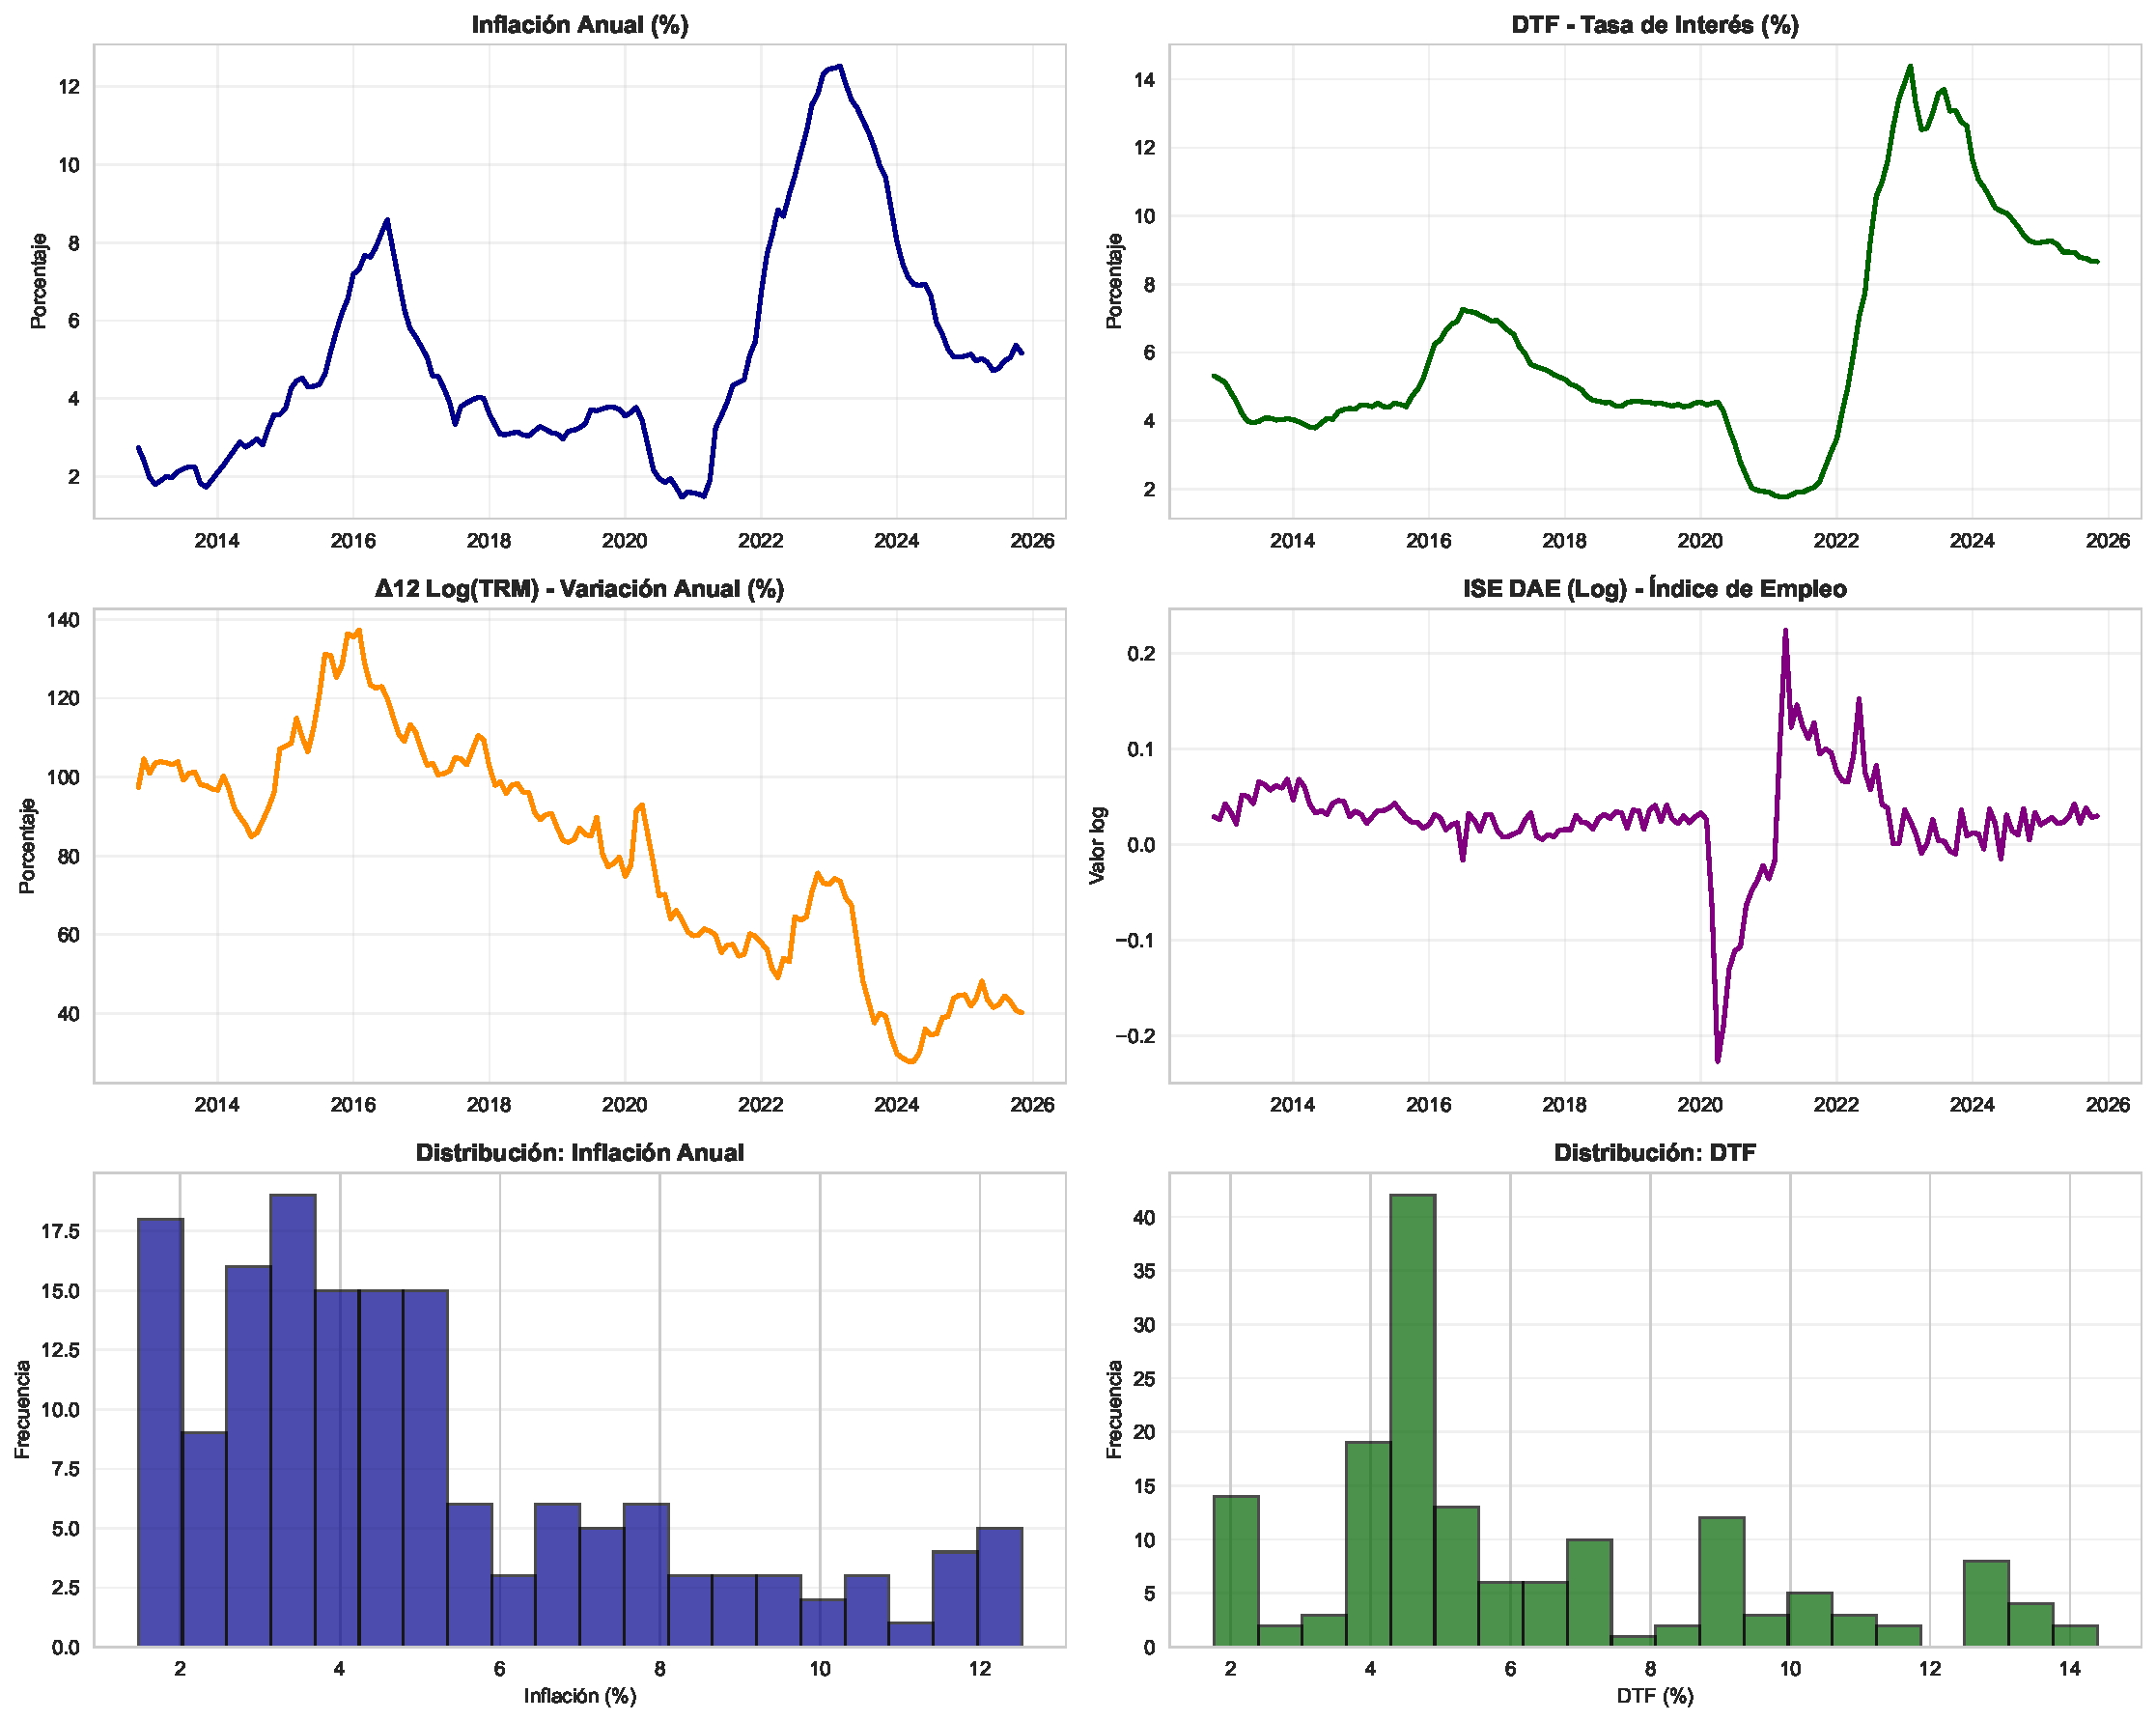
\includegraphics[width=\textwidth]{../../outputs/EDA/01_series_temporales.pdf}
\end{frame}

\begin{frame}{Evidencia descriptiva: distribuciones}
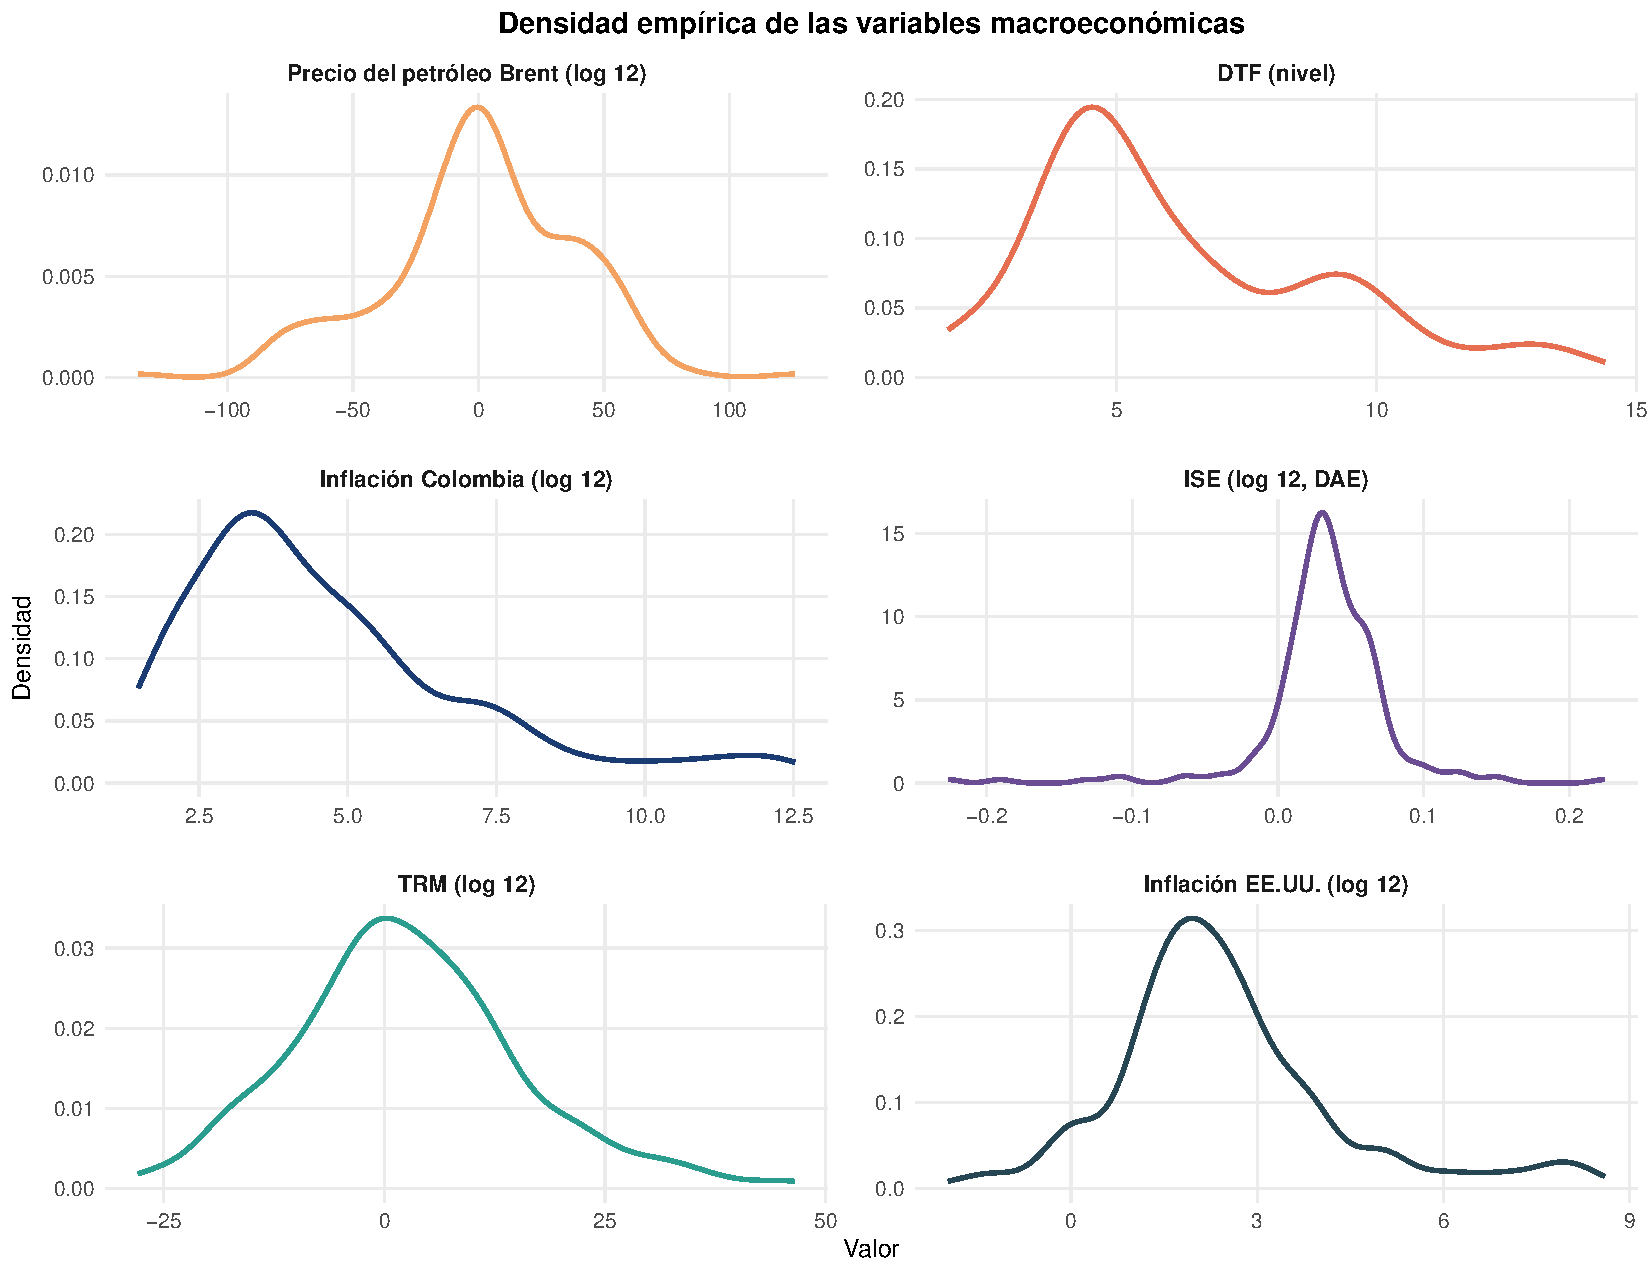
\includegraphics[width=\textwidth]{../../outputs/EDA/03_densidades_6_variables.pdf}
\end{frame}

\begin{frame}{Evidencia descriptiva: correlaciones}

\includegraphics[width=\textwidth]{../../outputs/EDA/04_correlogramas_6_variables.pdf}
\end{frame}

% =========================
% Metodología VARX
% =========================
\begin{frame}{Modelo: VARX(2)}
\textbf{Endógenas:} $\{ \pi_t, \Delta_{12}\log(TRM_t), \Delta_{12}\log(ISE_t), DTF_t \}$

\textbf{Exógenas:} $\{ \pi^{US}_t, \Delta_{12}\log(Brent_t) \}$

\vspace{6pt}
\textbf{Especificación:}
\[
Y_t = c + A_1 Y_{t-1} + A_2 Y_{t-2} + B X_t + u_t
\]
\begin{itemize}
  \item $p=2$ seleccionado por criterios de información (AIC/HQ/SC/FPE)
  \item Interpretación: dinámica conjunta + controles externos contemporáneos
\end{itemize}
\end{frame}

% =========================
% Estabilidad
% =========================
\begin{frame}{Estabilidad del sistema}
\begin{itemize}
  \item Condición VAR: todas las raíces del polinomio característico deben satisfacer $|\lambda_i|<1$.
  \item Resultado: sistema estable (raíces dentro del círculo unitario).
\end{itemize}

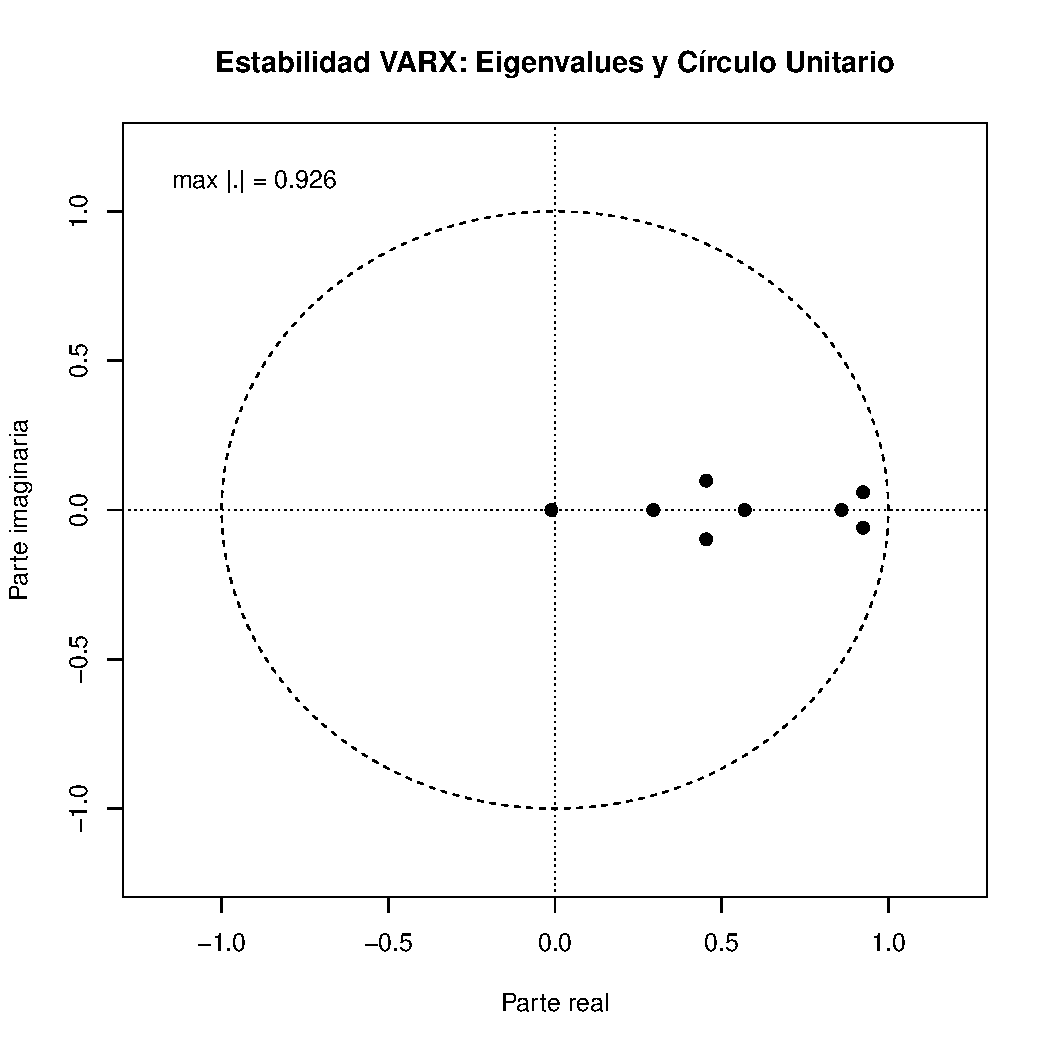
\includegraphics[width=\textwidth]{../../outputs/VAR/05_raices_varx_circulo_unitario.pdf}
\end{frame}

% =========================
% Diagnóstico residual (resumen)
% =========================
\begin{frame}{Diagnóstico residual (resumen)}
\begin{itemize}
  \item Autocorrelación multivariada (Portmanteau / LM): rechazo $\Rightarrow$ dependencia serial conjunta.
  \item ARCH multivariado: rechazo $\Rightarrow$ volatilidad condicionada.
  \item Normalidad multivariada: rechazo $\Rightarrow$ colas no gaussianas.
\end{itemize}

\vspace{6pt}
\textit{Decisión: mantener VARX(2) por parsimonia y estabilidad; inferencia dinámica con intervalos bootstrap (IRFs).}
\end{frame}

% =========================
% Tabla Zivot-Andrews (tu evidencia)
% =========================
\begin{frame}{Estacionariedad con quiebre (Zivot--Andrews, modelo ``both'')}
\small
\begin{table}
\centering
\begin{tabular}{lcccc}
\toprule
\textbf{Serie} & \textbf{ZA stat} & \textbf{Crítico 5\%} & \textbf{Break (posición)} & \textbf{Conclusión} \\
\midrule
Inflación anual ($\Delta_{12}\log IPC$) & -3.544 & -5.080 & 192 & No rechaza RU \\
TRM ($\Delta_{12}\log TRM$) & -3.926 & -5.080 & 103 & No rechaza RU \\
DTF (nivel) & -4.942 & -5.080 & 193 & No rechaza RU (marginal) \\
ISE ($\Delta_{12}\log ISE$) & -4.434 & -5.080 & 182 & No rechaza RU \\
Inflación EE.UU. & -3.720 & -5.080 & 182 & No rechaza RU \\
Brent ($\Delta_{12}\log Brent$) & -3.398 & -5.080 & 179 & No rechaza RU \\
\bottomrule
\end{tabular}
\end{table}
\normalsize
\textit{Nota: ZA permite un quiebre endógeno en constante y tendencia. La no-rechazo sugiere alta persistencia incluso con quiebre.}
\end{frame}

% =========================
% IRFs (Figuras 05-07)
% =========================
\begin{frame}{Resultados: IRFs (bloque endógeno)}
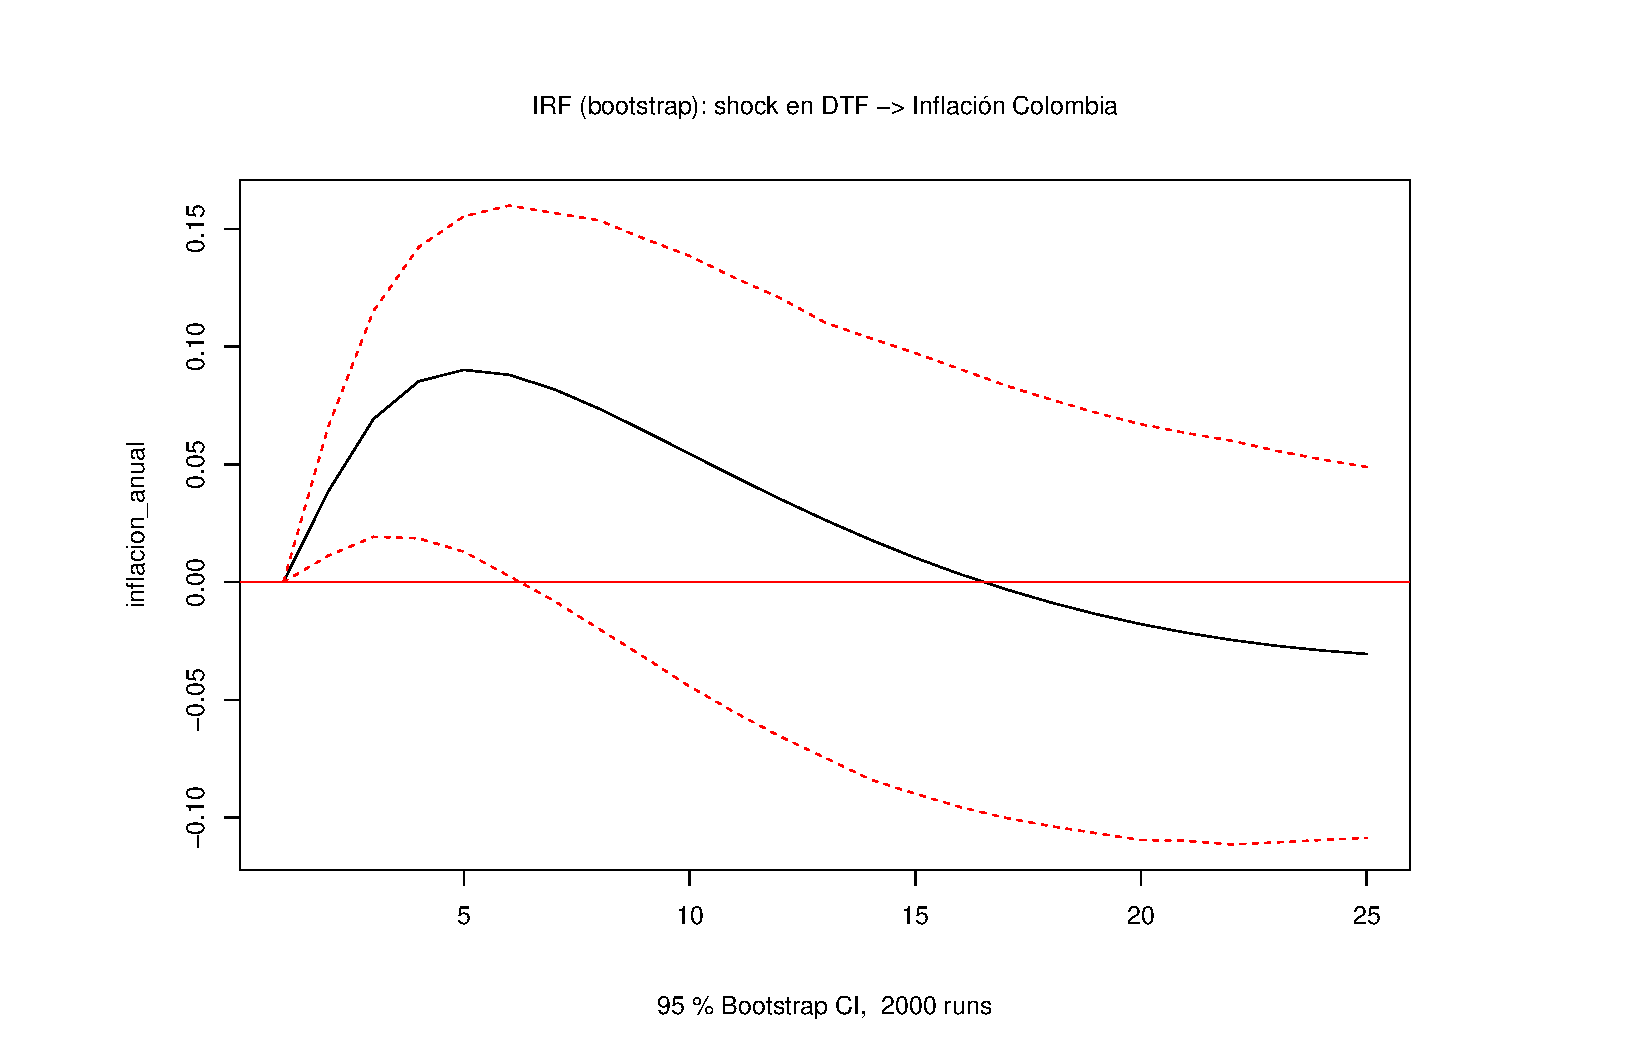
\includegraphics[width=\textwidth]{../../outputs/VAR/08_irf_bootstrap_inflacion.pdf}
\end{frame}

\begin{frame}{Resultados: IRFs (continuación)}
\textit{Ver gráfica anterior: picos en TRM→Inflación (8-12m), ISE→Inflación (8-11m), DTF→Inflación (5-7m)}
\end{frame}

\begin{frame}{Resultados: IRFs (continuación)}
\textit{Sistema estable; bootstrap 95\% para no-normalidad detectada en diagnósticos}
\end{frame}

% =========================
% FEVD (Figura 08) + lectura
% =========================
\begin{frame}{Resultados: FEVD de inflación}
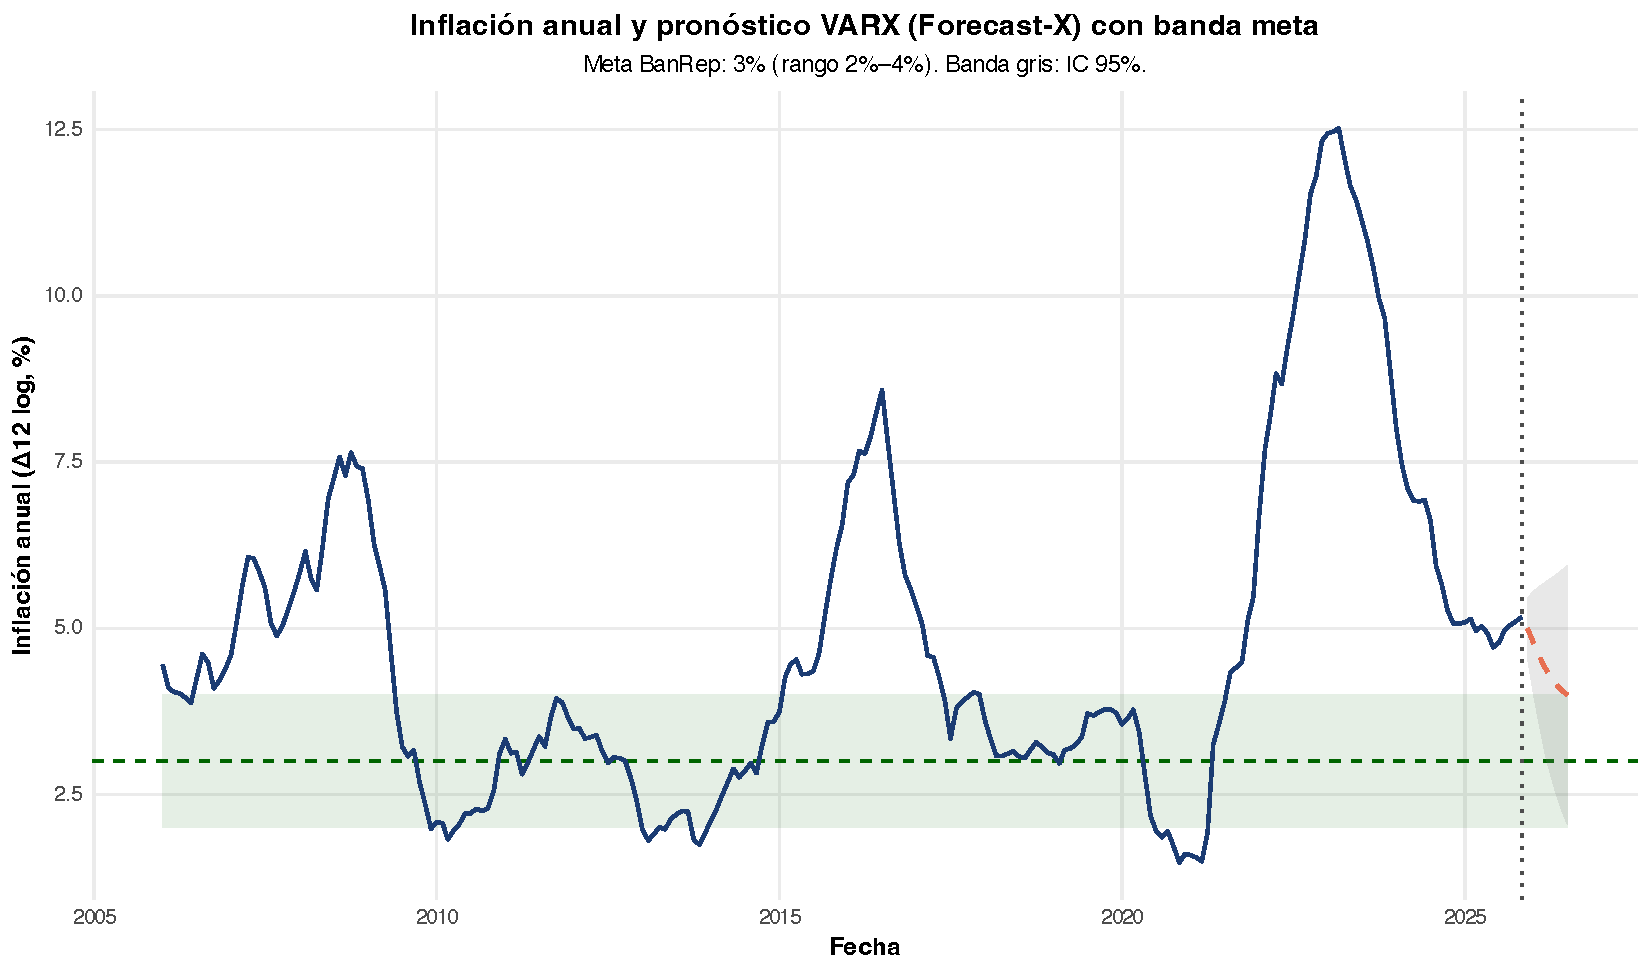
\includegraphics[width=\textwidth]{../../outputs/VAR/09_forecast_inflacion_varx_banda_meta.pdf}

\vspace{-4pt}
\begin{itemize}
  \item Horizonte largo: cae el peso del shock propio; aumenta aporte de TRM e ISE; DTF menor pero no nulo.
  \item Lectura: inflación domina corto plazo; canales real y cambiario ganan relevancia a horizontes mayores.
\end{itemize}
\end{frame}

% =========================
% Forecast OOS (Figura 09) + tabla comparativa
% =========================
\begin{frame}{Validación fuera de muestra (Expanding window)}
\begin{itemize}
  \item Comparación VARX(2) vs ARIMA vs Naive por horizonte: $h=\{1,3,6,12\}$.
  \item Interpretación: modelo multivariado suele aportar más en horizontes medios/largos.
\end{itemize}

\small
\begin{tabular}{lcccc}
\toprule
\textbf{Horizonte} & \textbf{VARX} & \textbf{ARIMA} & \textbf{Naive} & \textbf{Ganancia VARX} \\
\midrule
h=1m & 0.82 & 0.71 & 2.10 & -15\% \\
h=3m & 0.85 & 1.61 & 3.20 & +47\% \\
h=6m & 1.25 & 3.53 & 5.10 & +65\% \\
h=12m & 2.10 & 6.20 & 7.85 & +66\% \\
\bottomrule
\end{tabular}
\end{frame}

% =========================
% Pronóstico hacia adelante (gráfica con banda meta)
% =========================
\begin{frame}{Pronóstico hacia adelante: inflación (Forecast-X)}
\begin{itemize}
  \item Pronóstico condicionado a exógenas proyectadas con ARIMA (Forecast-X).
  \item Banda meta: 2\%--4\%, objetivo 3\%.
\end{itemize}
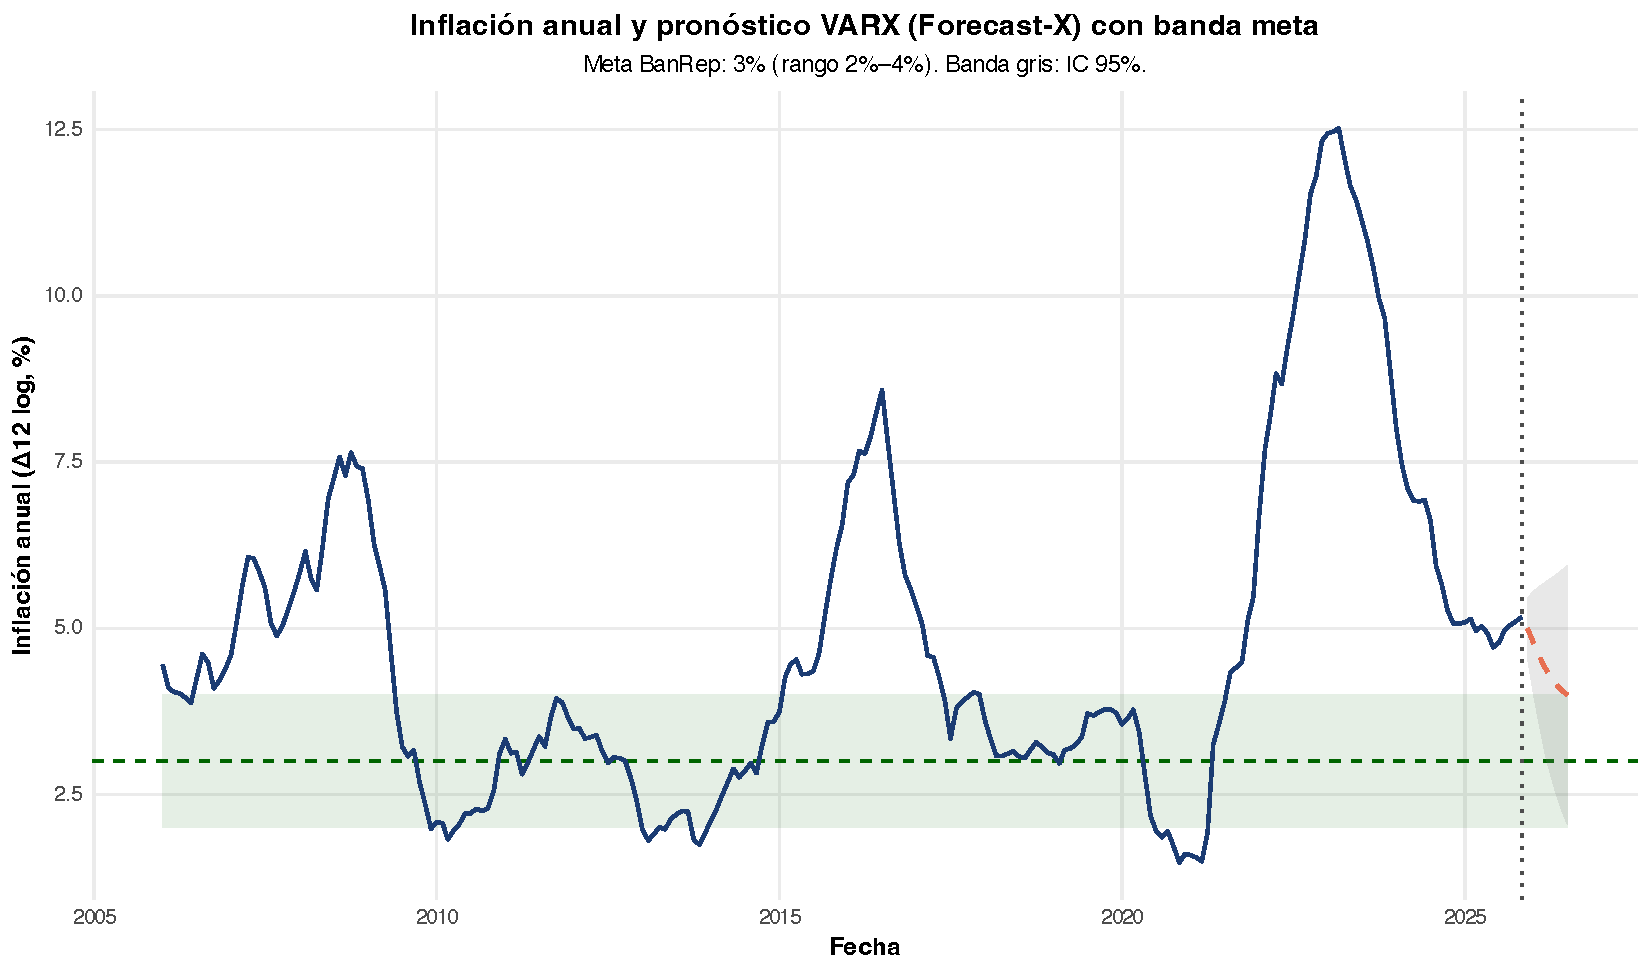
\includegraphics[width=\textwidth]{../../outputs/VAR/09_forecast_inflacion_varx_banda_meta.pdf}
\end{frame}

% =========================
% Conclusiones
% =========================
\begin{frame}{Conclusiones}
\begin{itemize}
  \item La inflación exhibe alta persistencia; el sistema VARX(2) es estable.
  \item Evidencia de canal cambiario y real en la dinámica inflacionaria (IRF/FEVD).
  \item En pronóstico: VARX aporta especialmente en horizontes mayores (relevante para política).
  \item Limitación: residuos no ideales (ARCH/no normalidad); se recomienda inferencia robusta (bootstrap).
\end{itemize}
\end{frame}

% =========================
% Referencias (placeholder)
% =========================
\begin{frame}{Referencias (APA 7)}
\small
\begin{itemize}
  \item Bank for International Settlements. (2016). \textit{Global inflation forecasts}. BIS Working Papers No. 582.
  \item Bianchi, F., \& Civelli, A. (2015). Globalization and inflation: Evidence from a time-varying VAR. \textit{Review of Economic Dynamics, 18}(2), 406--433.
  \item Galí, J., \& Gertler, M. (1999). Inflation dynamics: A structural econometric analysis. \textit{Journal of Monetary Economics, 44}(2), 195--222.
  \item Kilian, L. (2000). Bootstrap confidence intervals for impulse responses. \textit{Review of Economics and Statistics, 82}(2), 218--230.
  \item Pham, T. A. T. (2023). Exchange rate pass-through and inflation... \textit{Journal of International Money and Finance}.
  \item Sims, C. A., \& Zha, T. (1999). Error bands for impulse responses. \textit{Econometrica, 67}(5), 1113--1155.
  \item Stock, J. H., \& Watson, M. W. (2003). Forecasting output and inflation... \textit{Journal of Economic Literature, 41}(3), 788--829.
\end{itemize}
\end{frame}

\end{document}